\documentclass[../../main.tex]{subfiles}
\cite{gonardwikipedia}
\cite{gonardhistorischeslexikon}
\paragraph{}
\begin{figure}[h]
    \centering
    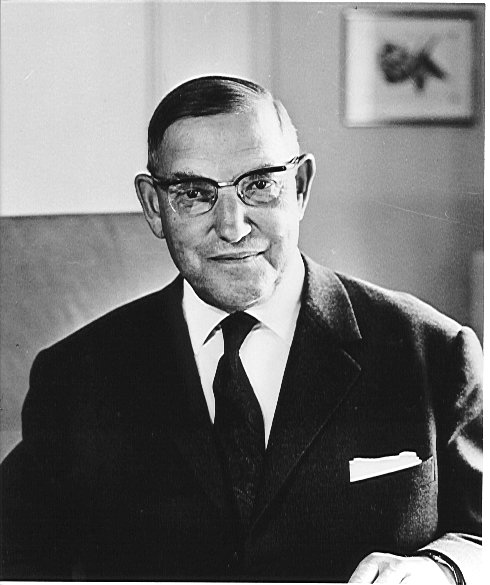
\includegraphics[width=\textwidth,height=7cm,keepaspectratio]{images/gonard.jpg}
    \caption{Samuel Gonard (unbekannt). Wikipedia. (10. Januar 2006). \newline URL: https://commons.wikimedia.org/wiki/File:Samuel\char`_Gonard.jpg Stand 16.07.2019}
\end{figure}
Samuel Gonard, geboren am 08. Juli 1896 in Neuenburg, ist der Sohn vom gleichnamigen Samuel Gonard, einem Händler. Samuel Gonard Junior war ein Schweizer Jurist und Berufsoffizier in der Schweizer Armee.
\paragraph{}
Samuel Gonard besuchte das Gymnasium in Neuenburg, später studierte er Rechtswissenschaften, das Studium schloss er 1921 ab. Von 1946 bis 1952 war er Dozent für Kriegsgeschichte und Taktik an der Eidgenössischen Technischen Hochschule in Zürich.
\paragraph{}
Bereits 1919 wurde er zum Leutnant in der Armee ernannt. In der Hierarchie stieg Gonard stetig empor, 1927 wurde er zum Hauptmann, 1933 zum Major befördert. Ab 1937 war er Mitglied der Generalstabsabteilung. 1939, dem Jahr des Kriegsbeginns, erhielt Gonard von General Guisan den Auftrag, seinen persönlichen Stab einzurichten und auch zu leiten. Vier Jahre später wurde Gonard zum Oberst-Brigadier und Unterstabschef der Armeeleitung ernannt, und war somit ein enger Mitarbeiter von Guisan. Der Plan der Reduitstrategie, der schlussendlich ausgeführt wurde, stammte von Samuel Gonard.
\paragraph{}
1961 wurde Gonard in das internationale Komitee des roten Kreuzes (IKRK) aufgenommen, kurz darauf beendete er seine Militärkariere. Von 1964 bis 1969 präsidierte Gonard das IKRK bis zu seinem altersbedingten Rücktritt.
\paragraph{}
Gonard war zweimal verheiratet, zuerst mit Hélène Dubois Gonard (ledig Louis), später mit Manon Bosshard Gonard (ledig Bosshard). Am 03. Mai 1975 verstarb Samuel Gonard 78-jährig in Corseau.